\documentclass{beamer}

\usepackage{préambule}

\begin{document}

\begin{frame}
	\begin{center}
		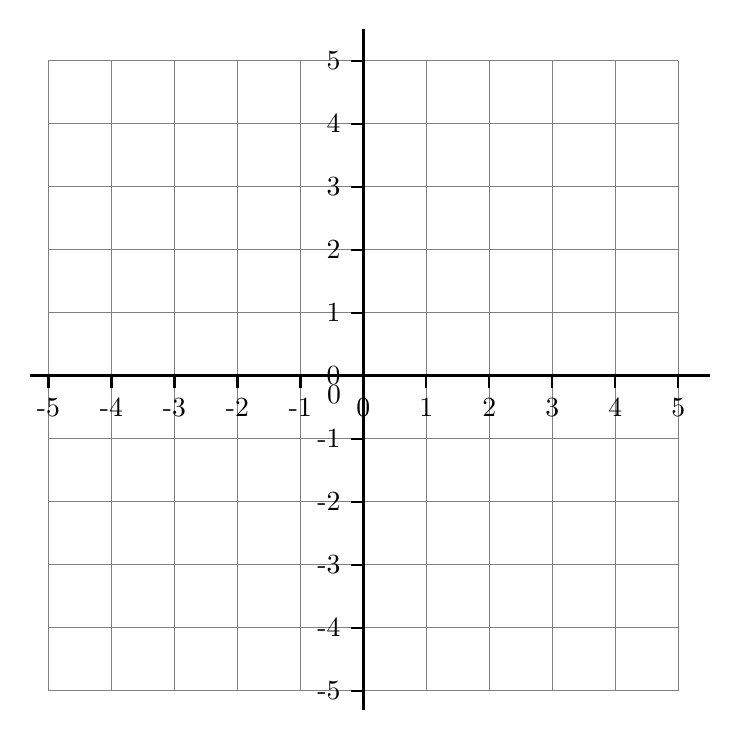
\begin{tikzpicture}[scale=0.8]
			\foreach \y in {-5, ..., 5} {
					\draw[thin,gray] (-5,\y) -- (5,\y);
					\ifthenelse{\equal{\y}{0}}{}{
						\draw[thick] (-0.2,\y) node[left] {\y} -- (0,\y);
					}
				}
			\foreach \x in {-5, ..., 5} {
					\draw[thin,gray] (\x,-5) -- (\x,5);
					\ifthenelse{\equal{\x}{0}}{}{
						\draw[thick] (\x,-0.2) node[below] {\x} -- (\x,0);
					}
				}
			\node[below,left] at (-0.2,-0.3) {$0$};
			\draw[very thick,\myArrow] (-5 - 0.3,0) -- (5 + 0.5,0);
			\draw[very thick,\myArrow] (0,-5 - 0.3) -- (0,5 + 0.5);
		\end{tikzpicture}
	\end{center}
\end{frame}

\end{document}